\section{Experiment and Results}

\subsection{Experiment Setup}

\subsubsection{Data Collection}

% TODO may need to update the last access date in ref.bib
% We use TWINT by \cite{twint} as our data collection tool.
% All the data can be accessed publically so there are no ethic considerations.

Numerous strategies considered in an attempt to procure data that belonged to
the war veterans. Transcripts of podcasts and YouTube videos involving accounts
of wars from the veterans, books that were written by the ex-servicemen, the
public dataset that had diaries, and letters of first world war soldiers were a
few sources. However, as an inference, all of these sources were highly specific
to the negative aspects and impacts of war and eventually would add bias to the
data.

On account of being a platform that is widely used by a large number of
service-men and the civilians, Twitter was selected as the platform to extract
data. Several verified Twitter pages linked to the US Army were manually analyzed
and a few profiles of the veterans were used as an initial set. Fitting
representation was ensured by selecting 6 veterans belonging to all the genders.
There was also no divide on the number of Tweets. The initial set had Twitter
profiles with as few as 57 tweets and as many as 39,000 tweets. The succeeding
veterans were picked by scouring through the followers of the veterans in the
original set based on some keywords like the army, us-army, military in their
bio.

A collection of 20 veterans was used for the initial proof of concept. However,
we intend to execute the study with 100 soldiers and 100 civilians.

Similarly, 6 civilians were selected with variations in age, sex, and the number
of tweets. The profiles from the initial set were later parsed to get random
followers. A collection of 20 commoners was used for the initial small-scale
proof of concept.

\subsubsection{Data Process and Analysis}

\begin{figure}[h]
  \centering
  \caption{Sequence of actions in the experiment}
  \label{pic:workflow}
  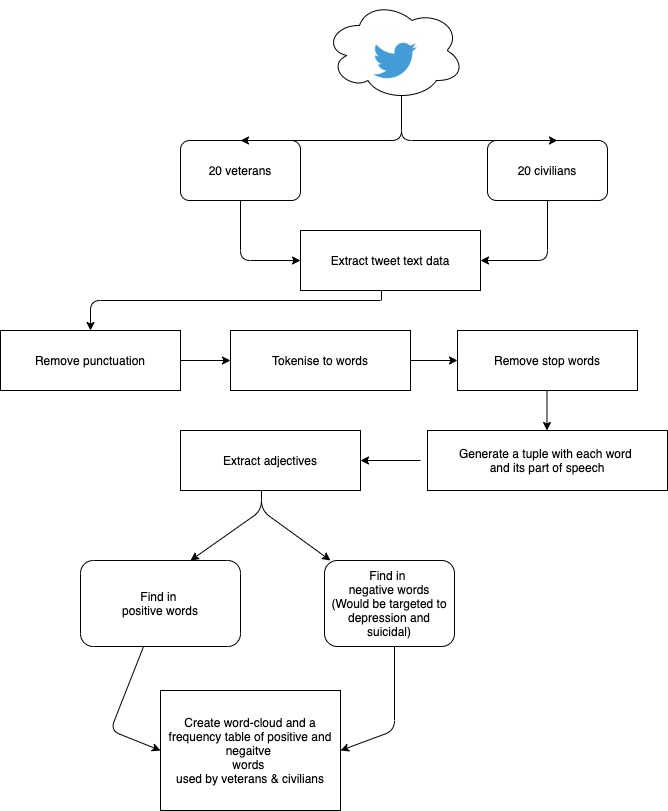
\includegraphics[width=0.75\textwidth]{twitter_workflow}
\end{figure}

Once the data is gathered and saved in the CSV format, we then start processing
the gathered data where we come up with a set of results to prove our
hypothesis. Sentiment analysis can be broadly categorized into two kinds, based
on the type of output the analysis generates. Under our processing, we are
trying to label text to be under \enquote{positive} and \enquote{negative}. Here we take into
account the tweets of all the selected veterans from our data and then run an
analysis to gather information of there sentiments breaking them into two parts,
that is word count of how much words they have used are under the world cloud
of being \enquote{Happy}, and the same for the one under \enquote{Sad}. This identical analysis
is then run on tweets by ordinary people. Finally, we will categorise these
words to check the two sets of results which will ultimately help us identify
an individual being in the state of depression with respects to the number of
words count of \enquote{positive} and \enquote{negative} results.

The initial step was to make a sack of remarkable words. One significant
perception that we went over was that not every one of a kind word is significant
for our handling. Thus, we focused on descriptive words which are profoundly
educational of positive and negative assessments. The next steps that we took
under processing our data were:

\begin{itemize}
  \item Removing punctuations
  \item Tokenizing
  \item Removing stop words
  \item Generating tuples
  \item Extracting the adjectives
\end{itemize}

The first step is to remove punctuation followed by Tokenizing which is the way
toward separating a goliath string into a rundown of words. \enquote{NLTK}, a python
library is used for this process. \enquote{Stop words}, where pull-out, as they do not
change any meaning of a sentence hence, can be ignored. Tuples were generated
with each word and ts part of speech. Finally, the adjectives were extracted
from the tweets of both the veterans and the civilians. And was then compared
with the word cloud that was created.

Finally, we compared the count of the positive and negative words used by the
two sets of people to come up with a result that displayed whether the veterans
were targeted to depression and suicidal.

The sequence of actions can be referred to Figure \ref{pic:workflow}.

\subsection{Results}
